\documentclass[11pt,a5paper]{article}

\usepackage[T1]{fontenc}
\usepackage[utf8]{inputenc}
\usepackage{lmodern, microtype}
\usepackage[estonian]{babel}
\usepackage{siunitx}
\sisetup{inter-unit-product=\ensuremath{{\cdot}}, per-mode=fraction, exponent-product=\cdot, output-decimal-marker={,}}
\usepackage{graphicx}
\usepackage{wrapfig}
\usepackage{adjustbox}
\usepackage{amsmath,amssymb}
\usepackage{amsfonts}
\usepackage[hidelinks]{hyperref}
\usepackage{csquotes}
\usepackage{caption}
\usepackage{enumitem}
\usepackage{soulutf8}
\topmargin=-3.0cm \textheight=19cm \textwidth=12.9cm
\oddsidemargin=-1.5cm  \evensidemargin=-1.5cm
\setlength{\parindent}{0pt} \setlength{\parskip}{6pt} \sloppy
\sloppy \relpenalty=10000 \binoppenalty=10000
\pagestyle{empty}

\newcommand{\numb}[1]{\vspace{5pt}\textbf{\large #1}}
\newcommand{\nimi}[1]{(\textsl{\small #1})}
\newcommand{\punktid}[1]{(\emph{#1~p.})}
\newcommand{\p}[1]{[\textbf{#1~p}]}
\newcounter{ylesanne}
\newcounter{expylesanne}
\newcommand{\yl}[1]{\addtocounter{ylesanne}{1}\numb{\theylesanne.} \nimi{#1} \newblock{}}
\newcommand{\expyl}[1]{\addtocounter{expylesanne}{1}\numb{E\theexpylesanne.} \nimi{#1} \newblock{}}
%\newcommand{\autor}[1]{}% Kasuta võistluse ajal
\newcommand{\autor}[1]{\emph{Autor: #1}}% Kasuta kui vaja autorit
\renewcommand{\leq}{\leqslant}
\renewcommand{\geq}{\geqslant}

\newenvironment{skeemlist}{\begin{itemize}[nosep, topsep=0pt, leftmargin=*]}{\end{itemize}}
\newenvironment{skeem}{\emph{Hindamisskeem}:\begin{skeemlist}}{\end{skeemlist}}

\begin{document}
\normalsize
\begin{center}
  \textbf{\Large Eesti koolinoorte 70.\ füüsikaolümpiaad} \par
  \emph{10.\ veebruar 2023. a. Piirkondlik voor.\\ Gümnaasiumi ülesannete lahendused (10.--12.\ klass)}
\end{center}

\normalsize

\numb{Eessõna}

Allpool on toodud iga ülesande üks õige lahenduskäik (mõnel juhul ka enam). \textbf{Kõik alternatiivsed õiged lahenduskäigud tuleb hinnata samuti maksimumpunktidega.} Iga alternatiivse lahenduskäigu jaoks tuleb kontrollijatel koostada hindamisskeem, juhindudes võimalusel juuresoleva hindamisskeemi punktijagamisproportsioonist. Soovituslikud mahaarvamise punktid:
\begin{skeemlist}
  \item numbriline arvutusviga --- \p{0,5};
  \item viga teisendustes --- \p{0,5} (märgi jms väiksem viga) või \p{1} (viga, mis viib dimensioonide konfliktini), maha arvata ainult üks kord, st edasikanduvat viga mitte karistada;
  \item kui vastus tuleb füüsikaliselt absurdne, siis võib täiendavalt karistada \p{0,5};
  \item üksik viga lähtevalemis --- \p{0,5} (kui märgiviga) kuni \textbf{50\%} (sisuline viga).
\end{skeemlist}
\vspace{1em}

\yl{VALGUSVIHK}
\punktid{6} \autor{Richard Luhtaru}

Kummagi juhu skeemid on toodud allpool. Mõlemal juhul läätsede fookused kattuvad, mistõttu valgusvihk jääb paralleelseks pärast läätsede läbimist.

\begin{figure}[h]
    \centering
    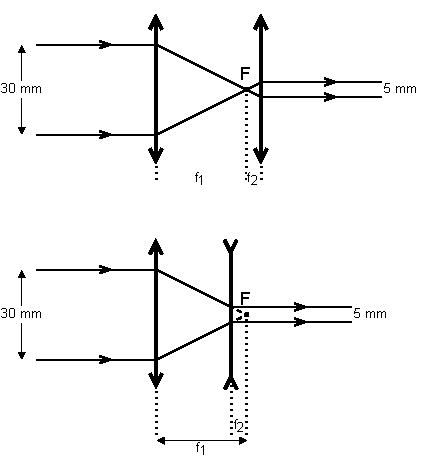
\includegraphics[width=.5\linewidth]{valgusvihk-lah.pdf}
\end{figure}

Sarnastest kolmnurkadest leiame, et kummalgi juhul $\frac{f_1}{f_2} = \frac{\SI{30}{mm}}{\SI{5}{mm}} = 6$. Ainsad Maril olevad läätsed, mille fookuskauguste suhe on $6$, on $\SI{12}{cm}$ ja $\SI{2}{cm}$. Seega esimesel juhul on Maril vaja kumerläätsi fookuskaugustega $\SI{12}{cm}$ ja $\SI{2}{cm}$. Teisel juhul on Maril vaja kumerläätse fookuskaugusega $\SI{12}{cm}$ ja nõgusläätse fookuskaugusega $\SI{2}{cm}$.

Tõestust, et teised läätsepaarid ei sobi, ei ole vaja.

\yl{OTSENE KALORIMEETRIA}
\punktid{6} \autor{Konstantin Dukatš}

Kui vesi voolab torus, siis vesi soojeneb inimeselt eralduva soojuse tõttu. Märkame, et aja $\Delta t$ jooksul siseneb väike vee element tuppa ja teine vee element samal hetkel väljub. Olgu $Q_i$ inimesest eralduv soojus aja $\Delta t$ jooksul ning $Q_v$ veele lisandunud soojusenergia. Energia jäävusest $Q_v = Q_i$ \p{1}.

Teame, et $Q_v = c\Delta m (T_2-T_1)$ \p{0,5} ja $Q_i = P\Delta t$ \p{0,5}, seega
$$c \Delta m (T_2 - T_1) = P\Delta t,$$
$$P = c \frac{\Delta m}{\Delta t} (T_2 - T_1).\quad\p{1}$$
Avaldame siseneva/väljuva vee elemendi massi
$$\Delta m = \rho \Delta V = \rho S u \Delta t. \quad\p{1}$$
Seega
$$P = c\rho S u (T_2-T_1),\quad\p{1}$$
$$P = \SI{4200}{\J\per\kg\per\celsius}\cdot \SI{1000}{\kg\per\m\cubed}\cdot \SI{e-4}{\m\cubed}\cdot \SI{2}{\m\per\s}\cdot\SI{0.15}{\celsius} = \SI{126}{\W} .\quad\p{1}$$


\yl{ÖKONOOMNE SÕIT}
\punktid{8} \autor{Marten Rannut}

Ülesandes pole vahet, kas leiame kütusekulude suhte $\SI{100}{\m}$ või $\SI{100}{\km}$ kohta \p{1} (juhul kui õpilane arvutab kütusekulud $\SI{100}{\km}$ jaoks, siis anda see punkt, kui õpilane leiab korrektselt $E_l$ $\SI{100}{\km}$ jaoks). Linnas kiirendab auto iga $\SI{100}{\m}$ tagant kiiruseni $v_l = \SI{40}{\km\per\hour} \approx \SI{11.1}{\m\per\s}$ \p{1}. Selleks kulub energia
\begin{equation*}
    E_l = \frac{mv_l^2}{2} = \frac{\SI{1500}{\kg}\cdot (\SI{11.1}{\m\per\s})^2}{2} \approx \SI{92.4}{\kJ}. \quad \p{1}
\end{equation*}

Maanteesõidul on auto kiirus $v_m = \SI{90}{\km\per\hour} = \SI{25}{\m\per\s}$ \p{1}. Auto poolt tehtav töö õhutakistuse ületamiseks on $E_m = Fs$ \p{1}, seega
\begin{equation*}
    E_m = cv^2s = \SI{1.3}{\kg\per\m}\cdot \left(\SI{25}{\m\per\s}\right)^2 \cdot \SI{100}{\m} \approx \SI{81.3}{kJ}.\quad \p{1}
\end{equation*}

Kuna mootori kasutegur on mõlemal juhul sama, siis kütusekulude suhe on võrdne kuluva energia suhtega \p{1}. Seega kütusekulude suhe on
\begin{equation*}
    \frac{k_m}{k_l} = \frac{\SI{81.3}{\kJ}}{\SI{92.4}{\kJ}} \approx \num{0.88}. \quad\p{1}
\end{equation*}
(või $k_l/k_m \approx \num{1.14}$).

\yl{DROON}
\punktid{8} \autor{Marten Rannut}

Tuule jõu muutus ajas on $\frac{\SI{25}{\N}}{\SI{0.7}{\s}} = \SI{35.7}{\N\per\s}$ \p{0,5}. Drooni jõu muutus ajas on $\frac{\SI{20}{\N}}{\SI{1}{\s}} = \SI{20}{\N\per\s}$ \p{0,5}. Järelikult resultantjõu muutus ajas on $\frac{\Delta F}{\Delta t} = \SI{35.7}{\N\per\s}-\SI{20}{\N\per\s}=\SI{15.7}{\N\per\s}$ \p{1}. Kuna $F=ma$, siis hakkab droon kiirenema, kusjuures kiirendus hakkab ühtlaselt kasvama \p{1}. Kiirenduse kasvamise kiirus on
\begin{equation*}
    \frac{\Delta a}{\Delta t} = \frac{1}{m}\frac{m\Delta a}{\Delta t} = \frac{1}{m}\frac{\Delta F}{\Delta t} = \frac{1}{\SI{0.5}{\kg}}\cdot \SI{15.7}{\N\per\s} = \SI{31.4}{\m\per\s\cubed}. \quad \p{1}
\end{equation*}

Teame, et kui keha algne kiirus on 0 ja kiirus hakkab kasvama ühtlaselt kiirendusega $a = \frac{\Delta v}{\Delta t}$, siis asukoha muutus on $\Delta s = \frac{at^2}{2} = \frac{\frac{\Delta v}{\Delta t}t^2}{2}$. Analoogselt, kuna kiirendus $a$ on kiiruse muutumise kiirus ja $\frac{\Delta a}{\Delta t}$ kiirenduse muutumise kiirus, siis ühtlase kiirenduse kasvamise korral $\Delta v = \frac{\frac{\Delta a}{\Delta t}t^2}{2}$ \p{3}. (Kui $\Delta v$ valemit pole leitud, aga on idee kasutada konstantse kiirenduse valemit $s = \frac{at^2}{2}$, siis \p{1}.)

Et drooni kiirus on algselt 0, siis drooni kiirus pärast $t=\SI{0.5}{\s}$ on
\begin{equation*}
    v = \Delta v = \frac{\frac{\Delta a}{\Delta t}t^2}{2} = \frac{\SI{31.4}{\m\per\s\cubed}\cdot (\SI{0.5}{\s})^2}{2} \approx \SI{3.93}{\m\per\s}
\end{equation*}
Numbrilise vastuse eest \p{1}.

\yl{VEDRU KEERUTAMINE}
\punktid{8} \autor{Sandra Schumann}

Olgu vedrude jäikused $k_1$ ja $k_2$, raskuste massid vastavalt $2m$ ja $m$, posti nurkkiirus $\omega$ ning vedrude algne pikkus $l$. Siis pikeneb esimene vedru pikkuse $2l - l = l$ võrra ja teine $4l - l = 3l$ võrra \p{1}. Esimese vedru pikenemisest tulenev jõud on $k_1 \cdot l$ ja teise vedru pikenemist tulenev jõud on $k_2 \cdot 3l$ \p{2}. Ringliikumisest saame ka, et esimese jõu suurus peab olema $2m \omega^2 \cdot 2l$ ja teise jõu suurus $m \omega^2 \cdot 4l$ \p{2}. Saame kirja panna, et:

$$k_1 \cdot l = 2m \omega^2 \cdot 2l$$
$$k_2 \cdot 3l = m \omega^2 \cdot 4l$$
$$\frac{k_1}{k_2} = \frac{2m \omega^2 \cdot 2l}{m \omega^2 \cdot 4l} \cdot \frac{3l}{l} = \frac{2 \cdot 2 \cdot 3}{4 \cdot 1} = 3$$

Vedrude jäikuste suhe on 3-kordne \p{3}.

\yl{KLAASPLAAT}
\punktid{10} \autor{Erkki Tempel}

\begin{center}
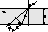
\includegraphics[width=0.5\linewidth]{klaasplaat_lahendus.pdf}
\end{center}
  
Kolmnurgast $\triangle{ABC}$ saame avaldada kiire nihke $BC$\\
\[ BC = AC \cos{\alpha} \quad \p{2}\]

Külje $AC$ pikkuse saame leida lõikude $AD$ ja $CD$ kaudu
\[ AC = AD - CD  \quad \p{1}\]

Avaldame külje AD kolmnurgast $\triangle{ADE}$
\[ AD = d\tan{\alpha} \quad \p{1}\]
Külje CD leidmiseks kasutame murdumisnäitaja seost
\[ \frac{\sin{\alpha}}{\sin{\gamma}} = n \quad \Longrightarrow \quad \sin{\gamma} = \frac{\sin{\alpha}}{n} \quad   \p{1}\]
Kolmnurgast  $\triangle{CDE}$ saame avaldada $\sin{\gamma}$ ning sealt külje $CD$
\[ \sin{\gamma} = \frac{CD}{CE} \quad \Longrightarrow \quad  CD = \frac{CE \sin{\alpha}}{n} \quad\p{1}\]

Kasutades eelnevat seost ning Phytagorase teoreemi kolmnurgast $\triangle{CDE}$,
saame avaldada külje CD
\[  CD = \frac{d\sin{\alpha}}{\sqrt{n^2-\sin^2{\alpha}}} \quad \p{2}  \]

Seega nihkub esialgne kiir kõrvale oma algsest sihist 

\[ BC = d\sin{\alpha}\left(1 - \frac{\cos{\alpha}}{\sqrt{n^2-\sin^2{\alpha}}}\right)  \quad \p{2}  \]

Kui lõppvastusesse on jäetud lihtsustamata trigonomeetriline pöördfunktsioon (nt $\arcsin$, $\arccos$), siis anda ülesande eest kuni \p{8}.

\yl{VOLTMEETER}
\punktid{10} \autor{Päivo Simson}

Olgu voltmeetri sisetakistus $R_v$. Skeemi sümmeetriast ja võrdusest $V_{AB}=V_{CD}$ järeldub, et takistused $R_1$ ja $R_3$ peavad olema võrdsed, st $R_3=R_1$. \p{1}

\begin{wrapfigure}{r}{0.35\textwidth}
\vspace{-1em}
  \begin{center}
    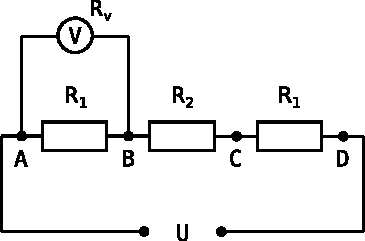
\includegraphics[width=1\linewidth]{ahelad_efo2.pdf}
  \end{center}
\end{wrapfigure}

1) Koostame kõigepealt skeemi, mis kujutab pinge mõõtmist punktide A ja B vahel. $R_v$ ja $R_1$ on ühendatud rööbiti ja takistus punktide A ja B vahel on järelikult
\[
R_{AB}=\frac{R_v R_1}{R_v + R_1}. \quad \p{0,5}
\]
Skeemi kogutakistus on
\[
R_{k}=\frac{R_v R_1}{R_v + R_1} + R_1+R_2. \quad \p{0,5}
\]
Pinge kahe punkti vahel jaotub proportsionaalselt nende punktide vahelise takistusega ja järelikult
\begin{multline*}
V_{AB}=U\cdot\frac{R_{AB}}{R_k}=\frac{U\frac{R_v R_1}{R_v + R_1}}{\frac{R_v R_1}{R_v + R_1} + R_1+R_2}=\\
=\frac{UR_vR_1}{R_v(2R_1+R_2)+R_1(R_1+R_2)}. \quad \p{1}
\end{multline*}

\begin{wrapfigure}{r}{0.35\textwidth}
\vspace{-1em}
  \begin{center}
    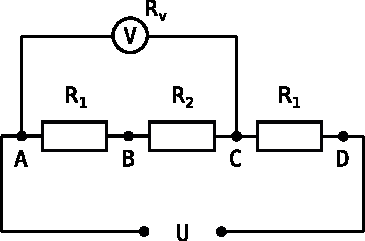
\includegraphics[width=1\linewidth]{ahelad_efo3.pdf}
  \end{center}
\end{wrapfigure}

2) Koostame skeemi, mis kujutab pinge mõõtmist punktide A ja C vahel. Analoogiliselt eelmise skeemiga saame
\[
R_{AC}=\frac{R_v (R_1+R_2)}{R_v + R_1+R_2}, \quad \p{0,5}
\]
\[
R_{k}=\frac{R_v (R_1+R_2)}{R_v + R_1+R_2}+R_1, \quad \p{0,5}
\]
\begin{multline*}
V_{AC}=U\cdot\frac{R_{AC}}{R_k}=\frac{U\frac{R_v (R_1+R_2)}{R_v + R_1+R_2}}{\frac{R_v (R_1+R_2)}{R_v + R_1+R_2}+R_1}=\\
=\frac{UR_v(R_1+R_2)}{R_v(2R_1+R_2)+R_1(R_1+R_2)}. \quad \p{1}
\end{multline*}

3) Paneme tähele, et $V_{AB}$ ja $V_{AC}$ murdavaldiste nimetajad on samad. Jagame need avaldised omavahel.
\[
\frac{V_{AB}}{V_{AC}}=\frac{R_1}{R_1+R_2}=\frac{28}{84}=\frac{1}{3} \quad\implies\quad R_2=2R_1. \quad \p{2}
\]
Asendades saadud tulemuse $V_{AB}$ avaldisse saame
\[
\frac{126 R_v}{4R_v+3R_1}=28\quad\implies\quad R_v=6R_1. \quad \p{2}
\]

\begin{wrapfigure}{r}{0.35\textwidth}
\vspace{-2em}
  \begin{center}
    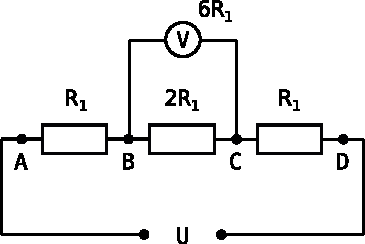
\includegraphics[width=1\linewidth]{ahelad_efo4.pdf}
  \end{center}
\vspace{-5em}
\end{wrapfigure}

4) Nüüd saame leida voltmeetri näidu $V_{BC}$. Vastavalt skeemile saame
\begin{multline*}
V_{AB}=U\cdot\frac{R_{BC}}{R_k}=\SI{126}{V}\cdot\frac{\frac{2R_1\cdot6R_1}{8R_1}}{\frac{2R_1\cdot6R_1}{8R_1}+2R_1}=\\
=\SI{126}{V}\cdot\frac{12}{12+8\cdot2}=\SI{54}{V}. \quad \p{1}
\end{multline*}

\yl{SÜVEND JA KERA}
\punktid{10} \autor{Marko Tsengov}

Juhul $\theta > \SI{90}{\degree}$ kukub kera kindlasti tasandilt maha.

Olgu $C \equiv \sqrt{(R - h)^2 + r^2}$. Kui $R = C$, siis puudutab kera korraga nii süvendi põhja kui ka äärt. Seega juhul $R > C$ puudutaks kera ainult süvendi äärt (mis pole ülesandes antuga kooskõlas).

Kui $R \leq C$, libiseb kera esmalt mööda süvendi põhja kauguse $C - R$ võrra, kogudes kineetilist energiat potentsiaalse energia arvelt. Seejärel kera põrkab servalt -- võib-olla korduvalt -- kuni ta kas ületab süvendi serva või jääb (aeglaselt sumbuvate põrkamistega) süvendisse. Selleks, et kera süvendist väljuks, peaks algne potentsiaalne energia olema suurem potentsiaalsest energiast, mille kera saavutab, kui see puudutab serva ning selle masskese on täpselt puutepunkti kohal. Teisisõnu peab kera sellises olekus olema madalamal kui algolekus. Kõrguste vahe saame leida, liigutades kera masskeskme mõtteliselt:
\begin{enumerate}
    \item Kera algsesse puutepunkti: $\Delta H = -R\cos\theta$
    \item Süvendi serva alumisse punkti: $\Delta H = -r\sin\theta$
    \item Süvendi serva ülemisse punkti (süvendi ääre peale): $\Delta H = h\cos\theta$
    \item Süvendi ääre kohale, nii et kera masskese on täpselt puutepunkti kohal: $\Delta H = R$
\end{enumerate}
Liites kõrguste vahed kokku, saame
\begin{equation*}
    \Delta H = -R\cos\theta - r\sin\theta + h\cos\theta + R = R-r\sin\theta-(R-h)\cos\theta
\end{equation*}

Kera saab süvendist väljuda, kui $\Delta H \leq 0$, st
\begin{equation*}
    R-r\sin\theta-(R-h)\cos\theta \leq 0
\end{equation*}

Ei ole oluline, kas õpilane kasutab tingimuses ranget ($<$) või mitteranget ($\leq$) võrratust.

\yl{SÜGAV KAEV}
\punktid{12} \autor{Jaan Kalda}

Vesi lõpetab kerkimise, kui see hakkab toru ülemises otsas keema, st küllastunud veeauru rõhk seal saab võrdseks atmosfäärirõhuga. Et temperatuuri tõustes küllastunud veeauru rõhk kasvab, siis vesi kaevu torus hakkab keema suurema rõhu juures, mistõttu veesamba kõrgus torus jääb väiksemaks.

Küllastunud veeauru rõhu saame leida vaadeldavatel temperatuuridel tänu sellele, et teame veeauru tihedust õhus ning õhu suhtelise niiskust. Kirjutame ideaalse gaasi olekuvõrrandi õhus oleva veeauru jaoks: $p_aV=\frac {m_a}\mu RT$ \p{1}, kus $p_a$ on veeauru osarõhk, $V$ on ruumala ja $m_a$ on selles ruumalas oleva veeauru mass. Jagades selle võrduse $V$-ga saame siduda rõhu ja tiheduse, $p_a=\frac {\rho_a}\mu RT$ \p{1}.

Küllastunud auru rõhk on leitav suhtelise õhuniiskuse definitsioonist: $p_k=p_a/r$ \p{1}, millest küllastunud aururõhu muutus $\Delta p_k=\frac {\rho_a}\mu R(T_1/r_1-T_2/r_2)$ \p{1}. Kaevutoru alumise otsa juures, kus põhjavee vaba pind on kontaktis atmosfääriga, on rõhk vees võrdne atmosfääri rõhuga $p_0$. Torus oleva veesamba ülemise otsa juures, kus toimub keemine, on rõhk torus väiksem veesamba tekitatud rõhu võrra, $p=p_0-\rho_v gh$ \p{1}, kus $h$ on veesamba rõhk. Et pumbates pumbatakse torust õhk välja ning asemele keeb veeaur, siis võime lugeda, et torus ongi puhas veeaur \p{2}, mille rõhk on võrdne küllastunud veeauru rõhuga antud temperatuuril, sest toimub keemine \p{2}, seega $p_k=p_0-\rho gh$. Et $p_0$ ei muutu, siis saame selle võrduse abil siduda veesamba kõrguse muudu küllastunud veeauru rõhu muuduga: $\Delta p_k=\rho g\Delta h$ \p{1}, kust saame, et
$$\Delta h=\frac {\rho_vR}{\mu\rho g}  \left(\frac{T_1}{r_1}-\frac{T_2}{r_2}\right)\quad\p{1}$$
ning numbriliselt $\approx \SI{14}{cm}$ \p{1}.

\newpage
\yl{ALAJAAMA KAUGUS}
\punktid{12} \autor{Jaan Kalda}

\begin{center}
    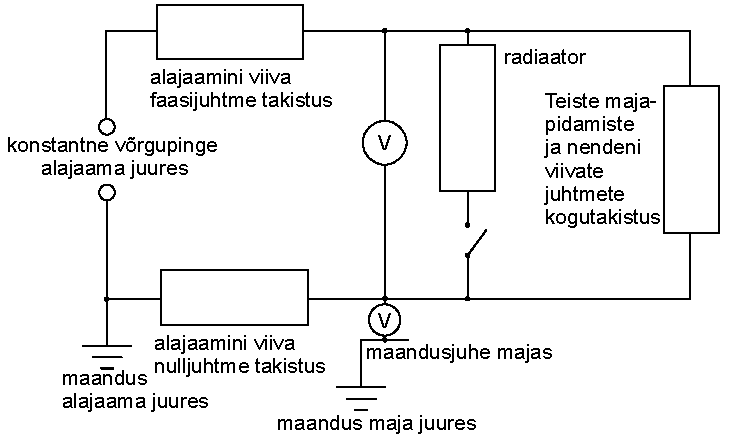
\includegraphics[width=0.8\linewidth]{alajaam_lah_joonis.pdf}
\end{center}

Kõigepealt teeme ekvivalentskeemi: radiaatori (takistusega $R_r$) ja teiste tarbijate (takistusega $R_t$) rööpühendus on järjestikku mõlema juhtmega pingeallika külge, milleks on alajaam; olgu kummagi juhtme takistus $R_j$ ja pinge alajaamas $U_a$. Selles skeemis on teada pinge ühel juhtmel $U_1$ ja pinge radiaatoril $U_f$; kui eemaldada skeemist radiaator, siis tekkiva uue olukorra jaoks on teada uus pinge juhtmel $U_0$. Kummagi ekvivalentskeemi eest saab \p{1}.

Esimesest ekvivalentskeemist saame Kirchoffi pingeseaduse tõttu 
$$U_a=U_f+2U_1;$$
see võrrand annab \p{2} (kui puudub tegur 2, siis \p{1}). 
Teisest ekvivalentskeemist saame tänu Kirchoffi pingeseadusele avaldada uue faasipinge, st pinge teistel koormistel:
$$U_f'=U_a-2U_0=U_f+2(U_1-U_0)=\SI{210}{\V} + 2(30-20)\,\si{\V} = \SI{230}{\V}.$$
see võrrand annab samuti \p{2} (kui puudub tegur 2, siis \p{1}).

Selleks, et leida juhtme pikkus, on meil esimese sammuna vaja leida juhtme takistus. Peale pingete avaldamist on meil on alles jäänud kolm tundmatut takistit, millest radiaatori takistuse saame avaldada tänu nominaalandmetele: 
$$P_n=U_n^2/R_r\;\; \Rightarrow\;\; R_r=U_n^2/P_n=\SI{26.45}{\ohm}.$$
See seos (emb-kumb) annab \p{1}. Kahe tundmatu leidmiseks vajame kahte võrrandit, milleks on Ohmi ja Kirchoffi seadustest tulenev järeldus: jadaühenduses jagunevad pinged võrdeliselt takistustega. Seega
$$U_0/U_f'=R_j/R_t,\quad\p{1}$$
$$U_1/U_f=R_j(1/R_t+1/R_r).\quad\p{1}$$
Lahutades teisest võrrandist esimese saame
$$U_1/U_f-U_0/U_f'=R_j/R_r\Rightarrow R_j=R_r(U_1/U_f-U_0/U_f')=\SI{1.479}{\ohm}.\quad\p{1}$$
Et $R_j=\rho L/S$ \p{1}, siis $L=SR_j/\rho\approx\SI{1920}{\m}$. Numbrilise vastuse eest \p{1}.

\end{document}